\chapter{First increment}
\label{chap:First Increment}
Test om: Bounce, predefined area
Skal komme væk fra accelerotmeter og gyroscope. 

\section{Requirements}
\label{sec:i1Requirements}
The requirements considered in this increment are marked with blue colouring.

\begin{itemize}
\item The trash bin should catch the trash if the user throws it towards the trash bin and within a predefined area
\begin{itemize}
\item \textcolor{blue}{The robots predefined area should be calculated from the hardware limitations of the motors’ speed}
\end{itemize}
\item The robot should know where it is positioned
\begin{itemize}
\item \textcolor{blue}{The robot should have a starting position, from where it should be able to calculate it's current position}
\item \textcolor{blue}{The robot's starting point should be placed outside its predefined area, such that it moves forward into the area}
\end{itemize}
\item The robot should be able to detect and track the thrown trash
\begin{itemize}
\item \textcolor{blue}{The thrown trash should be detected and tracked by a Microsoft Kinect}
\item The Kinect should send the coordinates of the impact point of the trash to the robot
\end{itemize}
\item The robot should know where the the thrown trash will land
\begin{itemize}
\item \textcolor{blue}{Trajectory prediction should be used to calculate impact point of the thrown trash}
%\item \textcolor{red}{The trajectory prediction should include a bounce prediction}
%\item \textcolor{red}{The bounce-shot should be thrown from a designated side of the camera}
%\item \textcolor{red}{The bounce-shot should bounce into the predefined area where the robot should catch the trash within }
\end{itemize}
\item The robot should be able to move the trash bin, such that the thrown trash lands inside the bin
\begin{itemize}
\item Multiple trash thrown should not be considered
\end{itemize}
\end{itemize}

These requirements are rudimentary, and the very essence of the project lies within the fulfilment of these requirements. In this increment the fundamentals of the robot’s movement should be implemented, the predefined area should be calculated, a starting point for this area should be determined and the Microsoft Kinect should be able to detect and track an object by using trajectory prediction.

\section{System design}
\label{sec:i1System Design}
The following sections describe how the marked requirements in \ref{sec:i1Requirements} will be attempted to be fulfilled. The theories and ideas behind will be explained subsequently.

\subsection{Predefined area}
\label{sec:i1Predefined area}
The robots predefined area, is an area where the robot should catch the ball within. This area is being made because of the limitations of the robots motors and is based on motor speed and average time of a throw, so the predefined area is where the robot should be expected to catch the ball within.

\subsection{Throwing}
\label{sec:i1Throwing}
The reason why the throw of the object (which in this project will be a table tennis ball) is important, is because the robot should have as much time to move to the collision point as possible. Before the robot moves to the collision point, the Kinect should calculate the where the robot should move, send the data to the robot, and the robot then moves. The Kinect can at any point send new data to the robot, so its course have to be changed, therefore it is important for the robot to have sufficient time to move within the predefined area.    

\subsection{Microsoft Kinect}
\label{sec:i1Microsoft Kinect}
To detect the thrown object, the Kinect has to use one of it's cameras, more specifically the depth sensor in this case. The depth sensor uses a range of infrared speckles, which draw a pattern in the room. Every cluster of speckles can be identified from each other, which makes the kinect able to differentiate between objects in the room. The depth of the specific object can be determined by the use of two cameras, as both cameras can identify the speckles at the object, it can triangulate the distance between the cameras and the object. This speckle pattern technology will only work indoor, and limits the use to only one kinect, as the speckles can be washed out by other lightsources.
\citep{kw}

\subsection{Trajectory prediction}
\label{sec:Trajectory prediction}
When the trash, referred to in this section as the projectile, is detected and the tracking of that projectile has started, the trajectory can be predicted. This prediction is limited to the amount of data sent by the sensory camera, meaning that for every camera reading, one detection of the object is gained. The precision of the prediction will increase according to the time a projectile has been tracked. \newline 
In this project, since the prediction is done indoor, the outdoor weather conditions that might affect the projectile trajectory is not considered. As well, the effects of air resistance, also called drag, will not be considered.

The trajectory of a projectile is the path of a thrown projectile without propulsion, affected by gravity. For calculating a trajectory of a projectile, the initial height, the angle which the projectile is launced from, the speed of the projectile at launch and the gravitational acceleration must be taken into account. \newline 
The initial height in this project is the height at which the projectile is detected, and the angle and speed at which the projectile is launched will be calculated from the first few trackings after detecting the projectile. The gravitational acceleration is considered as \(9.81m/s^2\), which is the standard near the earths surface. \newline
In this project we are interested in catching the projectile, and to do that, we need to calculate the distance the projectile travels before hitting the ground, and the amount of time before the projectile hits the ground. This is done with two mathematical formulas: \newline
\newline 
\begin{math}
g: \ the \ gravitational \ acceleration \ (9.81m/s^2)\newline
\theta: \ the \ angle \ at \ launch 
v: \ the \ speed \ at \ launch\newline
y_{0}: \ the \ initial \ height\newline
d: \ the \ total \ horizontal \ distance \ traveled \ \newline
t: \ the \ time \ of \ flight\newline
v_{vert}: \ the \ vertical \ velocity\newline
v_{hori}: \ the \ horizontal \ velocity\newline
t_{h}: \ the \ time \ since \ first \ detection\newline
d_{t}: \ the \ distance \ at \ time \ t\newline
\end{math}

From these variables we can express the formulas needed to provide the total distance traveled by the projectile, and the amount of time this would take.\newline
The distance traveled is:
\[d = \dfrac{v \ cos \ \theta}{g}(v \ sin \ \theta + \sqrt{(v \ sin \ \theta)^2 \ + \ 2gy_{0}})\] \newline
The time of flight is:
\[t = \dfrac{d}{v \ cos \ \theta} = \dfrac{v \ sin \ \theta \ + \ \sqrt{(v \ sin \ \theta)^2 \ + \ 2gy_{0}}}{g}\]
\newline

To calculate a trajectory of the projectile, the altitude and distance of the projectile at any time during the flight must be calculated, according to the initial height ( \(y_{0}\) ):
\[y = v_{vert}t - \dfrac{1}{2} gt^2\]
\[d_{t} = v_{hori}t\]

After this section, the projectile can be tracked, and the path for a given projectile can be calculated to a certain degree of correctness. 

\subsection{Gyroscope and Accelerometer}
\label{sec:i1Gyroscope and Accelerometer}
For positioning the robot, the Lego NXY Gyro and Accelerometer sensors will be considered. These sensors will be used together to position the robot, as the gyroscope will tell the number of degrees the robot has turned, which is relative to the heading of the robot at the start of the recording of data. This heading will be used together with an accelerometer, which can be used to calculate the distance the robot has traveled since the beginning of the recording of data. The time spent and the speed of the robot will be the data of this sensor.


\subsection{Movement}
\label{sec:i1Movement}
The robot was expected to be able to drive forward and backwards, to enable it to at most turn 90 degrees from any given angle, since any movement exceeding 90 degrees would be performed by driving backwards and turning from the opposite end of the robot. The robot was expected to be able to turn whether using either one active wheel or make both wheels go counterclockwise each other to turn more swiftly.


\section{Implementation}
\label{sec:i1Implementation}

\subsection{Gyroscope and Accelerometer in use}
\label{sec:i1Gyroscope and Accelerometer in use}
For the implementation of the gyroscope and the accelerometer, a test has to be done, to benchmark the precision of the sensors. For this, the data sent from the Arduino when the sensor has been plugged into the Arduino, was plotted in the Serial Plotter, which is a feature in the Arduino IDE. After various tests, the decision was to find a better alternative to these sensors, as the gyroscope in particular, had a lot of jitter. This jitter would even increase over time, making the use of the robot limited, as any user would have to restart the robot when the use wants to throw anything at the robot.

\subsection{Predefined area}
\label{sec:i1Predefined areaImplementation}
The robots predefined area will be calculated using the travel time of the ball and the speed of the motors used for the project. 
The predefined area was limited to be strictly in front of the robot as mentioned in movement.
As mentioned in  section \ref{sec:i1ThrowingImplementation}, the bouncing throw would have a travel time of 2 - 2.15 seconds, before landing in the predefined area. The predefined area was calculated using the robot itself. The robot was placed marking its starting point, which will always be its starting point. It was set to turn a specific number of degrees and move forward, after two seconds the robot would stop. The place the robot stops is marked aswell, which lead to the predefined area seen in figure \ref{figure:Predefined area}. The predefined area have an area of of 2851.5cm\begin{math}^2\end{math} which is 0.285m\begin{math}^2\end{math}.

\begin{figure}[h]
\centering
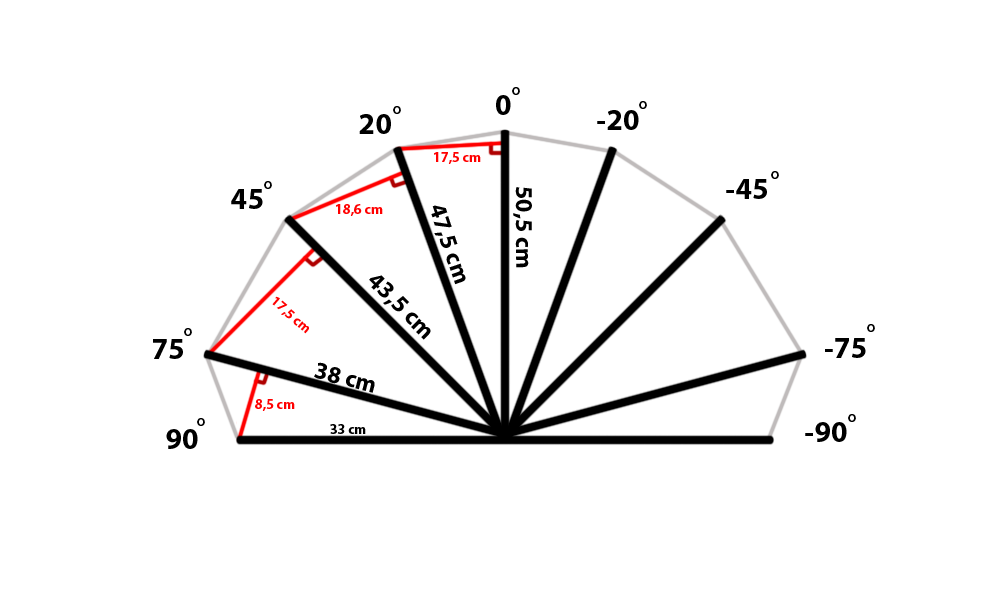
\includegraphics[scale=0.35]{billeder/predefined-area}
\caption{The robots predefined area}
\label{figure:Predefined area}
\end{figure}

\subsection{Throwing}
\label{sec:i1ThrowingImplementation}
Tests have been performed to ensure that the robot is provided the maximum amount of time for calculations and catching the trash. In order to do so, multiple test were conducted, and the results were acquired from a distance of 3 meter, the time it took for the trash (in this case, a table tennis ball) was in average 1.1 second. Multiple tests from a distance of 5 meter were also conducted and that provided an average of 1.25 second. 

With the results from the throwing tests, the group could conclude that a normal throw wouldn't provide enough time for the robot to catch the ball, else the predefined area for the robot had to be very small, due to the limitations of the motors. As mentioned in the \ref{sec:LEGO NXT Servo motor} section, the group calculated the robot's speed to be ~87 RPM, which simply isn't enough to catch trash from a 3 or 5 meter distance. The robot would be able to catch trash within 280mm of itself, given the 1.1 second run time of a 3 meter throw, and therefore nowhere near sufficient enough. 

The group decided after several tests to let the trash (still a table tennis ball) bounce on the floor before it had to be catched, which would give the robot extra time to get to the collision point of the ball. This provided nearly double the amount of time for the throw to be catched, providing an average of 2 seconds from a 3 meter throw and 2.15 seconds from a 5 meter throw.

\subsection{Microsoft Kinect}
\label{sec:i1Microsoft KinectImplementation}

\subsection{Gyroscope and Accelerometer}
\label{sec:i1Gyroscope and AccelerometerImplementation}

\subsection{Movement}
\label{sec:i1MovementImplementation}
Movement: The wheels were tested and forward motion was achieved with a speed of [insert speed] centimetres per second. The robot was also able to drive backwards at a lower speed of ….. Insert reason why we didn't turn by moving both wheels counterclockwise each other. It was discovered that the speed at which the robot drives backwards is much slower than its forward moving speed, because of the speed of backwards motion, it was decided to not consider driving backwards at all since the speed is inadequate (prefer tangible example) and since this would also simplify the problem. To solve this issue, it was decided to change the throw to always be in front of the machine, thus ensuring it would never be forced to drive backwards. This does however not take into account if the Kinect projectile prediction predicts the projectile will land behind the machine but this issue only arises if prediction is sufficiently miscalculated which is unlikely (anything else we can say about this? or rephrase).

\section{Evaluation}
\label{sec:i1Evaluation}
The requirements stating that the robot should know where it is positioned, will persist through this increment, as no solution has been found. The use of a gyroscope and accelerometer was not the right solution for this project, as the need of precise data would not be supported by sensors with a large amount of jitter. The robots starting position will always determine where the predefined area of the robot is, as the predefined area is defined by the robots position, and it's hardware limitations. The concept of predefined area is entirely based on the rotation speed of motor with wheel circumference and the duration of the throw, if any element the predefined area consists of changes, then so does the predefined area. Movement was not nearly as simple as expected and the implications of the problems encountered in its implementation is not fully solved in increment one.

When considering the the requirement: ”The robot should be able to turn, drive forward and drive backwards”, the group decided to remove the drive backwards part of the requirement as the group has decided to have a fixed starting point, from where the trash bin will always start and therefore didn’t see a reason for the ability to move backwards.
The other two parts of the requirement are fulfilled.

